\documentclass[presentation]{beamer}
\usepackage{common}

\title[\lecturecode{04}]{04 \\ Inheritance }

\author[Mirko Viroli]{Mirko Viroli}
\institute[]{\texttt{mirko.viroli@unibo.it}}

\begin{document}

\frame[label=coverpage]{\titlepage}
\newcommand{\codepath}[1]{../../code/lecture-04/#1}

\section{Reuse via inheritance}

\fr{Inheritance}{
  \bx{
    It is a mechanism that allows you to define a new class \alert{specialising} an existing one, that is, ``inheriting'' its members (the private ones are not directly visible), possibly modifying / adding new members, and therefore reusing code already written and tested.
  }
  \bl{Inheritance is a key concept of OOP}{\iz{
    \item It is related to the interface mechanism
    \item It is one of the key elements along with encapsulation and interfaces
    \item It not only affects code reuse, but also the resulting polymorphism
  }}
}


\frs{5}{Reuse and extension scenarios}{
  \bl{Scenarios}{\iz{
    \item Given a class, create another with only partially different (or new) characteristics
    \item Given a class, create a more specialised one (for example, more robust and secure even if less performing, or vice versa, more performing)
    \item Create hierarchies of classes or behaviors, to model hierarchical domains
    \item A library could be structured as framework: to use it you have to extend certain classes it provides
  }}
  \bl{An example we develop upon}{\iz{
    \item usual class \cil{Counter}
    \item want to evolve and have also a \cil{MultiCounter} -- with many incremements at once
    \item to avoid repetition, could use delegation, and will then explore inheritance
  }}
}

\fr{Basic example: \Cil{Counter}}{
\codeview{1}{5}{25}{\scriptsize}{\codepath{Counter/Program.cs}}
}

\fr{A new class: \Cil{MultiCounter}}{
\codeview{1}{5}{29}{\ssmall}{\codepath{MultiCounter/Program.cs}}
}

\fr{Version with reuse via composition/delegation}{
  \codeview{1}{19}{34}{\ssmall}{\codepath{MultiCounterWithDelegation/Program.cs}}
}

\frs{15}{The need to extend and modify}{
  \bl{A typical situation}{\iz{
    \item It is typical in software projects to find that you have to create modified versions of existing classes -- it is a natural evolution situation
    \item Relying on the ``copy and paste'' code is \alert{always} inadvisable (DRY principle), because it tends to scatter errors throughout the code, and complicates maintenance
    \item Getting reuse via composition (i.e. delegation) is generally a \alert{good solution}, but there are alternatives with certain advantages
  }}
  \bl{The inheritance mechanism is used}{\iz{
    \item Definition: \cil{class C : D \{.. \}}
    \item The new \cil{C} class inherits all members of \cil{D}{\iz{
      \item The private members are not directly accessible from within \cil{C}
      \item The constructors of \cil{D} must always be rewritten, and should properly call \cil{C}'s
    }}
    \item Terminology: \cil{D} superclass, or base class, or parent class
    \item Terminology: \cil{C} subclass, or child class, or specialization
    \item Note: it is not necessary to have the \cil{D} sources, the binary code is enough, in fact in the future we will extend library classes without having the source
  }}
}

\fr{A new version of \Cil{MultiCounter}}{
  \codeview{1}{18}{29}{\scriptsize}{\codepath{MultiCounterInheritance/Program.cs}}
}

\fr{Rational}{
  \bl{We redefine the \cil{MultiCounter} class as an extension of \cil{Counter}}{\iz{
    \item We define the new method \cil{multiIncrement()} by just adding it
    \item We define the necessary constructor{\iz{
      \item The constructor of a subclass should have the \cil{base} statement, which calls a (non-private) constructor of the parent class
      \item If it doesn't, the parent's default constructor is called (if existing)
      \item Without constructors, you usually have only the default one
    }}
  }}
  \bl{The meaning of the definition}{\iz{
    \item An object of \cil{MultiCounter} is similar to an object of \cil{Counter}{\iz{
      \item Has method \cil{Increment()} and property \cil{Value}, both inherited
      \item It also has the (implicit) value field (which is actually incremented), although its setter is private, hence it is inaccessible from the \cil{MultiCounter} class code (\cil{Value++} would not work!)
    }}
    \item Two necessary changes with respect to \cil{Counter}: \cil{MultiIncrement ()} method and constructor
  }}
}

\fr{UML notation for extension}{
  \bx{\iz{
    \item Solid line arc (points to full triangle) for the relation ``\cil{extends}''
    \item Arcs grouped to improve graphic rendering
  }}
  \fg{width = 0.45 \textwidth}{img/uml-ext.pdf}
}

\fr{UML notation - simplified version for design}{
  \fg{width = 0.4 \textwidth}{img/uml-ext2.pdf}
}


\frs{8}{\Cil{protected} access level }{
  \bl{Usable for the members of a class}{\iz{
    \item It is an intermediate level between \cil{public} and \cil{private}
    \item Indicates that the member (field, method, constructor, property) is accessible from the current class, from a subclass, and from subclasses of subclasses (recursively)
  }}
  \bl{What is it for?}{\iz{
    \item It allows subclasses to access supra-class information that you don't want clients to see
    \item Most often used in retrospect replacing a \cil{private}
    \item Using \cil{protected} fields is to be avoided -- it somewhat breaks encapsulation; should better use \cil{protected} properties/methods
  }}
  \bl{Example class \cil{BiCounter} - bidirectional counter}{\iz{
    \item A counter with also the \cil{Decrement} method
    \item Impossible without making the \cil{Value} accessible also for modification
  }}
}

\fr{\Cil{ExtendibleCounter} and \Cil{BiCounter}}{
  \codeview{1}{5}{34}{\tiny}{\codepath{BiCounter/Program.cs}}
}

\fr{Analogous solution with fields}{
  \codeview{1}{18}{38}{\ssmall}{\codepath{BiCounterFields/Program.cs}}
}

\frs{20}{Overriding}{
  \bl{Extension and modification}{\iz{
    \item When creating a new class by extension, it is very often not enough to add new functionality
    \item Sometimes it is also necessary to modify some of those available, possibly even distorting a bit their original functioning
    \item This can be done by rewriting in the subclass one (or more) of the methods/properties of the superclass -- called an \alert{override}
    \item To do so, methods/properties in the base class must be declared \cil{virtual}, and those in the subclass \cil{override}
    \item If necessary, the rewritten method can invoke the version of the parent using the special receiver \cil{base}
    \item It is possible to ``hide'' a method in the superclass that is not \cil{virtual}, by the modifier \cil{new} -- but this mechanis is optional, and arguably with limited use
    \item A class can be declared \cil{sealed} to prevent extension
    
  }}
  \bl{Example \cil{LimitCounter}}{\iz{
    \item Create a (sealed) counter which, having reached a certain limit, no longer continues
    \item It is necessary to override the \cil{Increment()} method
    \item An additional getter method inspects when the limit is reached
  }}
}

\fr{Using the \Cil{LimitCounter} class}{
  \codeview{1}{5}{18}{\scriptsize}{\codepath{LimitCounter/Program.cs}}
}


\fr{Class \Cil{LimitCounter}}{
  \codeview{1}{20}{41}{\scriptsize}{\codepath{LimitCounter/Program.cs}}
}

\fr{UML notation}{
  \bx{\iz{
    \item Protected members are annotated with a ``\#''
    \item The overridden methods are also reported in the subclass
  }}
  \fg{height = 0.6 \textheight}{img/uml-ext3.pdf}
}

\fr{A summary of access modifiers (for types and members)}{
    \bx{Recall that \cil{internal} means ``visible only in this assembly''}
    \bl{Who can access?}{\iz{
        \item \cil{public}: any other code in the same assembly or another assembly that references it
        \item \cil{private}: only by code in the same class
        \item \cil{protected}: only by code in the same class, or in a class that is derived from that class
        \item \cil{internal}: by any code in the same assembly, but not from another assembly
        \item \cil{protected internal}: by any code in the assembly in which it's declared, or from within a derived class in another assembly
        \item \cil{private protected}: only within its declaring assembly, by code in the same class or in a type that is derived from that class
    }}
}

\fr{Class \Cil{Object}}{
    \bl{Implicit extension of \cil{Object}}{\iz{
        \item when a class extends nothing, it is like extending \cil{System.Object}
        \item transitively, this means all classes inherit from \cil{Object}
        \item it provides low-level services for all objects 
        \item we will in the following explain some of them
    }}
    \bl{Method \cil{String ToString()}}{\iz{
        \item it can be overriden to provide a canonical string representation of an object
        \item \cil{Console.Write} uses it if you try to write an object
    }}
}

\section{A complete scenario}

\fr{An application to the smart home automation scenario}{
   \bl{Elements}{\iz{
     \item We use \cil{LimitCounter}
     \item We define a \cil{LimitedLamp} (via extension) which contains a counter, and which has a life time based on the number of allowed switches to on
     \item A \cil{SmartHomeController} consists of $n$ \cil{LimitedLamp}s, and has the ability to check if all the lamps are exhausted, and to switch on the lamp that has the most life left
   }}
} 

\fr{Whole UML Diagram}{
  \fg{height=0.8\textheight}{img/uml-domus.pdf}
}

\fr{SmartHomeController: expectation}{
  \codeview{1}{106}{128}{\ssmall}{\codepath{SmartHome/Program.cs}}
}


\fr{Counters}{
  \codeview{1}{5}{26}{\scriptsize}{\codepath{SmartHome/Program.cs}}
}

\fr{Devices}{
  \codeview{1}{27}{56}{\tiny}{\codepath{SmartHome/Program.cs}}
}

\fr{SmartHomeController pt.1}{
  \codeview{1}{58}{76}{\ssmall}{\codepath{SmartHome/Program.cs}}
}

\fr{SmartHomeController pt.2}{
  \codeview{1}{78}{104}{\ssmall}{\codepath{SmartHome/Program.cs}}
}

\section{On virtual methods}

\frs{5}{Analyse this code}{
    \codeview{1}{5}{32}{\ssmall}{\codepath{Analysis/Program.cs}}
}

\fr{A similar case: \Cil{UnlimitedCounter}}{
    \codeview{1}{12}{35}{\ssmall}{\codepath{UnlimitedCounter/Program.cs}}
}

\fr{Explanation of virtual methods}{
    \bl{What happens when calling \cil{Increment()} on an \cil{UnlimitedCounter}?}{\iz{
     \item Not having an override, the version in \cil{LimitCounter} is used
     \item Within \cil{LimitCounter},\cil{IsOver()} is called  which itself calls \cil{ToLimit()}
     \item The executed version of \cil{ToLimit} is that of \cil{UnlimitedCounter}
   }}
   \bl{A general rule of OOP}{
      When a virtual method is called (from inside or outside an object), the version actually used is the most specific available for the receiver of the invocation!
   }
   \bx{This is achieved thanks to the so-called ``virtual methods table''}
}

\fr{The virtual methods table}{
     \bl{Also called: vtable, call table, dispatch table}{\iz{
        \item each class \cil{C} has one such table, and all its objects have a reference to it
        \item for each virtual method defined (or inherited) in \cil{C}, the vtable associates the corresponding code to execute, that is the class that defines the body
        \item the calls to be resolved with this table are those with \alert{late binding}
        \item it is a structure that makes polymorphism between classes efficient (which we will see)
     }}
     \bl{Example}{
        How are the tables related to the \cil{LimitedCounter} and \cil{UnlimitedCounter} classes in the previous example?
     }
}

\fr{Memory management example: stack / heap / vtables}{
   \fg{height = 0.8 \textheight}{img/layout.pdf}
}

\section{Inclusive polymorphism with classes}

\frs{15}{Inheritance and polymorphism}{
  \bl{Remembering the principle of substitutability, we can say:}{
    If \texttt{B} is a subtype of \texttt{A} then any object of \texttt{B} can be used (and ``must'' be usable) where an object of \texttt{A} is expected
  }
  \bl{With inheritance}{\iz{
    \item With the definition: \cil{class B : A \{.. \}}
    \item Objects of class \cil{B} can reply to all messages expected by class \cil{A}, and possibly to a few more
    \item So an object of class \cil{B} could be passed where one of class \cil{A} is expected, without causing problems (of ``typing'')
  }}
  \bl{Consequence:}{
    Since it is possible, correct, and useful, then in C\# (and in all other mainstream OOP langs) class \cil{B} is treated as a subtype of \cil{A} in all respects!
  }
  \bl{A side note}{
    However, some pursists argue that substitutability would better left to interfaces only, and use inheritance for reuse only
  }
}

\fr{Polymorphism with classes}{
\fg{width = 0.7 \textwidth}{img/uml-poli.pdf}
}

\fr{Polymorphism with classes}{
  \bl{In a class \cil{D} that uses a class \cil{C}}{\iz{
    \item there will be points in \cil{D} where objects of class \cil{C} are expected
    \item (as arguments to methods, or as type of fields)
    \item you can actually pass objects of the class \cil{C}, but also of the classes \cil{C1}, \cil{C2}, .., \cil{C5}, or any other subsequently created class that extends, directly or indirectly, \cil{C}
  }}
  \bl{Subclasses of \cil{C}}{For all intents and purposes, objects of subclasses of \cil{C} are compatible with objects of class \cil{C} \iz{
    \item have the same contract (in general, possibly a few more operations)
    \item have all fields defined in \cil{C} (in general, a few more)
    \item hopefully have compatible behavior (Liskov principle)
  }}
}

\frs{10}{Layout of objects in memory}{
  \bl{Some aspects of the layout of objects in memory \dots}{
    Let's give some general and abstract information (the specific .NET version could manage objects a little differently). However, many elements are common.
  }
  \bl{Structure of an object in memory}{\iz{
    \item Starts with a header inherited from \cil{Object} (few bytes), which includes{\iz{
      \item Indication of which class of the object is (runtime type information)
      \item Table of method pointers, to support late-binding
      \item The (private) fields of the \cil{Object} class (if any)
    }}
    \item Gradually all the fields of the class, starting with those of the superclasses, going down the hierarchy
  }}
  \bl{Consequences: If the \cil{C} class is a subclass of \cil{A} ...}{
    Then an object of \cil{C} is similar to an object of \cil{A}, it only has additional information at the bottom, and this makes substitutability easier!
  }
}

\fr{Example polymorphism between classes - UML}{
  \fg{height = 0.8 \textheight}{img/uml-person.pdf}
}

\fr{\Cil{UsePerson} and \Cil{Person}}{
  \codeview{1}{5}{34}{\tiny}{\codepath{Person/Program.cs}}
}

\fr{Specialisations of \Cil{Person}}{
  \codeview{1}{36}{58}{\tiny}{\codepath{Person/Program.cs}}
}

\frs{5}{Differences with polymorphism of interfaces}{
  \bl{Polymorphism with interfaces}{\iz{
    \item A class \cil{D} uses objects via an interface \cil{I}, not another class \cil{C}
    \item It can be assumed that there is a certain contract, but not that there is a specific behavior (that of \cil{C}) that has possibly been specialized -- in fact, who cares?
  }}
  \bl{Classes do not allow ``multiple inheritance'' (only C++ actually does)}{\iz{
    \item It is NOT possible in C\# to declare: \cil{class C : D1, D2}{\iz{
      \item problems would arise if \cil{D1} and \cil{D2} had common properties
      \item it would become difficult to manage the in-memory structure of the object
    }}
    \item With interfaces there are no such problems, and as a result:{\iz{
      \item it is much easier to take an existing class and make it compatible with an interface, rather than a class
      \item recall that we could always use interfaces for polymorphism, and inheritance/delegation for reuse
    }}
  }}
}

\fr{Summary of inclusive polymorphism}{
  \bl{Polymorphism}{\iz{
    \item Provides supertypes that collect common partes of classes
    \item Can support highly-reusable components
    \item Useful for building homogeneous collections of objects
  }}
  \bl{Polymorphism with interfaces}{\iz{
    \item Relative to a contract only
    \item Ease of joining existing classes to the contract
    \item There is often a tendency to create a large number of interfaces
  }}
  \bl{Polymorphism with classes}{\iz{
    \item Relating to contract and behaviour
    \item Typically need construction ``from the start''
    \item Constrained by single inheritance
  }}
}


\section{Types at run-time}

\fr{Everything is an \Cil{Object}}{
   \bl{Why having a common root for all classes?}{\iz{
     \item Allows you to factor common behavior
     \item Allows the construction of functionalities that work on any object
   }}
   \bl{Application examples:}{\iz{
     \item Polymorphic containers, for example via array of type \cil{object[]}{\iz{
       \item allows you to build a list of objects of a different nature
     }}
   }}
} 

\fr{Polymorphism with \Cil{object}}{
  \codeview{1}{5}{29}{\ssmall}{\codepath{PolyObject/Program.cs}}
}

\frs{5}{Static type and run-time type}{
  \bl{A duality introduced by subtyping (inclusive polymorphism)}{\iz{
    \item Static type: the data type of an expression that can be inferred by the compiler
    \item Run-time type: the data type of the value (/ object) actually present (could be a subtype of the static one, and can be inspected with \cil{GetType()}){\iz{\item in this case virtual method calls rely on late-binding}}
  }}
  \bl{Example in \cil{PrintAll()} code, inside the \cil{foreach}}{\iz{
    \item Static type of \cil{obj} is \cil{Object}
    \item Run-time type of \cil{obj} varies from time to time: \cil{String}, \cil{Int32}, \dots
  }}
  \bl{Type inspection at run-time}{\iz{
    \item In some cases it is necessary to inspect the type at run-time
    \item The case of the \cil{is} and \cil{as} operators
    \item However, using them is bad practice: it means you have poorly used polymorphism
  }}
}

\fr{Type check and conversion}{
  \codeview{1}{6}{32}{\tiny}{\codepath{PersonRuntime/Program.cs}}
}

\section{Abstract classes}

\frs{5}{Motivations of abstract classes}{
  \bl{Between interfaces and classes}{\iz{
    \item Interfaces describe only one contract
    \item Classes define complete behavior
    \item \dots is there room for intermediate constructs?
  }}
  \bl{Abstract classes}{\iz{
    \item They are used to describe classes with partial behavior, i.e. in which some methods are described but not implemented
    \item These classes cannot be instantiated (the \cil{new} operator cannot be used)
    \item Can be extended and completed in subclasses, and there we can have generation of objects
  }}
  \bl{Typical application: pattern Template Method}{
    It is used to declare a strategy scheme with a method that defines a common behavior (often non-virtual), but which uses methods to be concretised in subclasses
  }
}

\frs{5}{Abstract classes}{
  \bl{An abstract class:}{\iz{
    \item is declared as such: \cil{abstract class C ... \{\... \}}
    \item it cannot be used to generate objects
    \item can optionally declare abstract methods/properties: \iz{
      \item they have the form, for example: \cil{abstract int m (int a, String s);}
      \item i.e. without body, as in interface declarations
    }
  }}
  \bl{Other aspects}{\iz{
    \item can define fields, constructors, methods, properties 
    \item \dots must carefully define their access level
    \item can extend from an abstract or non-abstract class
    \item can implement interfaces, without having to comply with the contract
    \item a class extending an abstract one can be non-abstract only if it implements all defined methods
  }}
}

\frs{5}{Example: \Cil{FailingLamp} as an abstract class}{
  \bl{Objective}{\iz{
    \item We want to design a lamp extending \cil{Device} with the concept of exhaustion/failure
    \item The strategy with which to manage this exhaustion can be varied
    \item But you have to make sure that whatever strategy you specify, it is guaranteed that:{\iz{
      \item the lamp turns on only if not exhausted
      \item in the event of actual activation, it is possible to keep track of it, for strategic purposes
    }}
  }}
  \bl{Solution}{\iz{
    \item Careful use of \cil{abstract}, \cil{virtual}, and \cil{protected}
    \item We will give three possible specializations for a \cil{FailingLamp}{\iz{
      \item that never runs out
      \item that runs out at the n${}^{th}$ switch on
      \item that runs out after a certain time from the first switch on
    }}
  }}
}

\fr{overall UML}{
  \fg{height = 0.8 \textheight}{img/uml-abstract.pdf}
}

\fr{\Cil{FailingLamp}}{
  \codeview{1}{5}{29}{\ssmall}{\codepath{FailingLamp/Program.cs}}
}

\frs{5}{Specialisations}{
  \codeview{1}{31}{62}{\tiny}{\codepath{FailingLamp/Program.cs}}  
}

\fr{Wrap-up on inheritance}{
   \bl{The more general case:}{
     \cil{class C : D, I, J, K, L \{.. \}}
   }
   \bl{What the \cil{C} class should / can do}{\iz{
     \item must implement all methods declared in \cil{I, J, K, L} and super-interfaces
     \item can override (non-final) methods defined in \cil{D} and superclasses
   }}
   \bl{Abstract class:}{
     \cil{abstract class CA : D, I, J, K, L \{.. \}}
   }
   \bl{What the \cil{CA} class should / can do}{\iz{
     \item is not required to implement any methods
     \item can implement some method to define partial behavior
   }}
} 

\end{document}



\fr{Possible errors related to conversions}{
  \bl{Semantic errors (compile-time, therefore harmless)}{\iz{
    \item Conversion attempt that is neither upcast nor downcast
    \item Call to a method not defined by the receiver (static) class
  }}
  \bl{Execution errors (very dangerous, avoidable with \cil{instanceof})}{\iz{
    \item Downcast to a class incompatible with the dynamic type, reported as \cil{ClassCastException}
  }}
  \srcode{\scriptsize}{3}{30}{\ecl / last / ShowCCE.java}
}

\fr{\Cil{instanceof}, conversions and \Cil{Person}}{
  \sizedrangedcode{\scriptsize}{3}{100}{\ecl / person / UsePerson2.java}
}




\end{document}

\fr {Outline} {
  \bl {Goal of the lesson} {\iz {
  \item Describe general concepts of encapsulation, information hiding, composition, reuse
  }}
  \bl {Technical arguments} {\iz {
  \item the \cil{interface} construct
  \item substitutability (and subtyping)  
  }}
}

\section{Decomposition, encapsulation, information hiding}

\fr{The principle of decomposition}{
\bx{\Huge divide et impera}
\bl{Divide and conquer: \alert{top-down} approach}{\iz{
  \item The solution of a complex problem occurs by dividing it into simpler, independent problems
  \item Subdivision is often multi-level
}}
\bl{Example}{\iz{
\item Smart home controller: GUI, event management, algorithms to manage devices
\item Management software: People management, Tasks management, GUI, Interaction with DB
}}
}

\fr{Decomposition, modularity and dependencies}{
  \bl{A crucial point of decomposition is ``modularity''}{\iz{
    \item The division must be done in such a way that it is actually convenient
    \item The simpler ``subproblems'' need to be isolated
    \item This is possible if we minimize the ``dependencies'' between the subproblems, which allows:
   {\iz{
      \item more decision-making autonomy
      \item less interaction with others
      \item \alert{less negative influences in case of changes}
    }}
  }}
}

\fr{Modularity: which situation is preferable?}{
\begin{center} 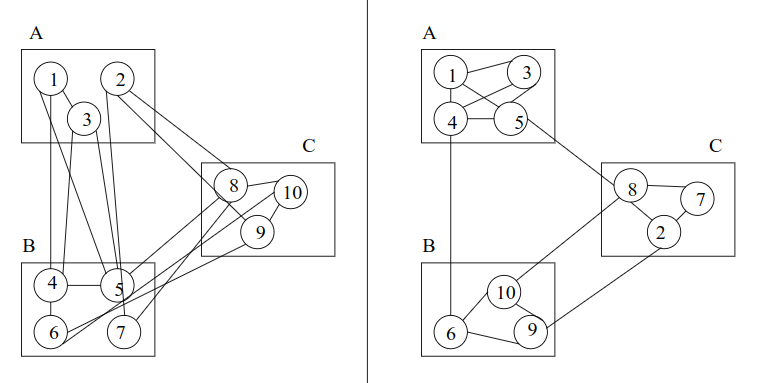
\includegraphics[height=0.6\textheight]{img/coupling.png} \end{center}
}

\frs{10}{Decomposition and OO programming}{
  \bl{In OO programming, we have several levels of decomposition}{\en{
    \item Subdivision into projects (of the entire program)
    \item Subdivision into namespaces (of the entire project)
    \item Subdivision into classes (of a namespace)
    \item Subdivision into methods (of a class)
  }}
  \bl{The crucial point to be addressed now is the division into classes}{\iz{
    \item You must divide your code into classes as appropriate
    \item Creating the best link with the problem space
    \item \alert{Reducing dependencies between classes as much as possible}
  }}
  \bl{Technique}{\iz{
    \item There are well-established efficient programming techniques that solve this problem, which we will begin to explore in this lesson - getting it right takes some time and experience!
  }}
}

\fr{Dependencies and OO}{
  \bl{Dependence}{
    A class \cil{A}  is said to depend on a class \cil{B}  if within the code of \cil{A} the class \cil{B}, or some of its members, are mentioned or used. The dependency is deeper if many constructors/fields/methods/properties defined in \cil{B} are used in \cil{A}.
  }
  \bl{Implication}{
    Each dependency strongly constrains the possibility of making changes, because it involves others to be made in cascade. If \cil{A} depends on \cil{B} and I modify \cil{B}, I will probably have to modify \cil{A} as well.
  }
  \bl{The ``untouchability'' syndrome --- rigid SW}{
    When building complex software with too many unneeded dependencies, you get to the point that every single change would require many more, and therefore they become too expensive - as a result, you end up refusing change at all!
  }
}

\frs{5}{Encapsulation}{
  \bl{Two crucial ingredients of OO programming}{\en{
    \item Packing data + functions to manipulate it
    \item Information hiding via careful access control
  }}
  \bl{Philosophy}{\iz{
    \item Each class declares \cil{public} only those (few) methods/properties/constructors necessary to interact with (or create) its instances
    \item The rest (which therefore includes mere implementation aspects) is \cil{private}{\iz{
      \item methods/constructors/properties for internal use only
      \item{\bf{all}} fields (i.e. internal status)
    }}
  }}
  \bl{Encapsulation and dependencies}{In this way the ``client'' is weakly influenced by possible future modifications concerning mere implementation aspects.
  }
}

\frs{5}{A basic case: class \Cil{Counter}}{
    \codeview{1}{18}{40}{\scriptsize}{\codepath{Counter/Program.cs}}
}

\fr{A basic case: usage of class \Cil{Counter}}{
    \codeview{1}{5}{16}{\scriptsize}{\codepath{Counter/Program.cs}}
}

\frs{5}{Counter usage} {
  \bl{The \cil{Counter} class} {\iz{
   \item Encapsulates simple counting functionality
   \item Gives a more abstract and modular approach than using directly an \cil{int}
   \item Allows you to act on the count only with \cil{GetValue()} and \cil{Increment()}
   \item [$\Rightarrow$] it is impossible to change the counter at will (or by mistake), for example by decreasing instead of increasing, or by zeroing
  }}
   \codeview{2}{44}{55}{\scriptsize}{\codepath{Counter/Program.cs}}
}

\frs{10}{Counter usage, and evolvability} {
  \bl{An evolution scenario for \cil{Counter}} {\iz{
   \item Case: Assume want to change counting of elements: up to a certain limit counting should stop
   \item The below solution is still valid, by just changing the internal implementation of class \cil{Counter}
   \item Note it is crucial that the client uses \cil{Increment} instead of making \cil{\_countValue} public
  }}
   \codeview{2}{44}{55}{\scriptsize}{\codepath{Counter/Program.cs}}
}


\fr{Reflection: encapsulation and contract}{
  \bl{Contract}{\iz{
    \item The contract of an object corresponds to its usage scenarios
    \item And therefore to the expectations that a customer has when using the object
    \item Thanks to encapsulation, it is possible to strongly constrain these contracts, better controlling the behavior of objects
  }}
  \bl{The case of the Counter}{\iz{
    \item The value of the count at the time of construction is \cil{0}
    \item The count value at any other time is equal to the number of calls to \cil{Increment()}
  }}
  \bl{Observation}{
    It is thanks to this idea that it is easier to compose objects in more complex systems
  }
}

\fr{Encapsulation is preserved by properties!}{
    \codeview{1}{5}{30}{\ssmall}{\codepath{CounterProperties/Program.cs}}
}

\fr{A modification to the counter implementation}{
    \codeview{1}{33}{52}{\ssmall}{\codepath{CounterProperties/Program.cs}}
}

\fr{Properties vs methods vs fields: recap}{
    \bl{``Properties are just methods''}{\iz{
        \item a read-only property is essentially a Getter
        \item a read-write property is essentially a pair of Getter and Setter method
        \item most discussions in the following focus on methods, and applicability to properties naturally derive
    }}
    \bl{``Properties define a nice abstraction''}{\iz{
        \item from the design viewpoint, public properties are much nicer than Getters/Setters, which are still the OOP standard
    }}
    \bl{``Properties can replace fields''}{\iz{
        \item as an implementation mechanism, auto-implemented properties are a good replacement for fields
        \item but this is just matter of internal implementation
    }}
}

\section{A methodology based on encapsulation}

\fr{Another example: class \Cil{Lamp}}{
  \bl{Problem analysis}{
    In a smart home automation system, we will have to manage a certain number of lamps (to be switched on/off and controlled via a special centralised application, e.g., via a smartphone). These are push-button commands with intensity control (10 levels). The controller must be able to access the state of each lamp (on/off, intensity level) and modify it as desired. At the first start, the lamps are off and the intensity control is at zero (in a range of $[0,1]$).
  }
  \bx{How do we build the \cil{Lamp} class?}
}

\fr{Design and implementation: phases}{
  \bl{Modern steps in building a class}{\en{
    \item Design of the public part of the class
    \item Definition of a test for the class
    \item Definition of the state 
    \item Implementation completion
    \item Test the result
    \item Final code improvement
  }}
}

\fr{Phase 1: Design of the public part of the class}{
  \bx{That is, the name of the class and the signatures of public operations (methods and constructors)}
  \bl{Guidelines}{\iz{
    \item Consider all the various use cases of an object of the class
    \item Insert constructors and public methods only for necessary operations
    \item Where possible, avoid entering a large number of such operations
  }}
  \bl{The \cil{Lamp} case}{\iz{
    \item A unique constructor with no arguments
    \item Methods for turning on / off
    \item Methods for increasing / decreasing / setting intensity
    \item Methods for accessing the state of the lamp
  }}
  
}

\fr{Public part -- a skeleton}{
    \codeview{1}{24}{39}{\footnotesize}{\codepath{LampInterface/Program.cs}}
}

\fr{Phase 2: Definition of a test}{
\bx{That is, expectations}
  \bl{In general}{\iz{
    \item this amount to the general problem of testing prior to coding
    \item we will in the future study in detail the test-driven approach
    \item specific technologies and methods will be used for testing
  }}
  \bl{In our specific case for the \cil{Lamp} case}{\iz{
    \item we consider a main program calling some methods on a lamp object
    \item it is not a deep test, but, properly expanded, could be a good starting point
  }}
}

\fr{Test code}{
    \codeview{2}{8}{21}{\footnotesize}{\codepath{LampInterface/Program.cs}}
}

\frs{5}{Phase 3: Definition of the state}{
  \bx{That is, private fields of the class}
  \bl{Guidelines}{\iz{
    \item Consider that there are various possible choices (it is an implementation aspect, which can be retracted later)
    \item The set of fields must be as small as possible, due to performance (memory space) and non-duplication needs
    \item The set of fields must be sufficient to keep track of all the ways in which the behavior of the object can change in the face of messages received
  }}
  \bl{The \cil{Lamp} case}{\iz{
    \item We will need to know if it is on or off (\cil{bool \_on})
    \item We will need to know the current intensity level (\cil{double \_intensity})
    \item No more information seems to be needed, at this point... we'll see later
  }}
}


\fr{Phase 4: Implementation completion}{
\bx{That is, the body of constructors and methods}
  \bl{Guidelines}{\iz{
    \item Realise the body of each constructor and method in a way compatible with the contract provided for the class
    \item Accept that the first version produced will not necessarily be the final version
  }}
  \bl{The \cil{Lamp} case}{\iz{
    \item \cil{On()}, \cil{Off()} are simple Setters-like methods
    \item \cil{IsOn()}, \cil{GetIntensity()} are simple Getters-like methods
    \item \cil{Dim()} and \cil{Brigthen()} modify the \cil{\_intensity} field (if in range!)
  }}
}

\fr{First Lamp Class version}{
  \codeview{1}{23}{50}{\tiny}{\codepath{LampFirst/Program.cs}}
}

\fr{Phase 5: Final code improvement}{
  \bl{Guidelines}{\iz{
    \item Insert comments into the code only if needed
    \item Verify the need for constants to avoid ``magic'' numbers
    \item Eventually factor sub-functions into public/private methods/constructors, to avoid duplication
    \item Possibly consider using public properties as well
  }}
  \bl{Specifically in this case}{\iz{
    \item There are magic numbers, use constants!
    \item The constructor is the default one
    \item Better manage the $0..1$ limit
    \item Avoid intermediate levels ($0.145$) of brightness
    \item Retract the type choice of the \cil{\_intensity} field -- it is better to have internally an \cil{int} between $0$ and $10$!!
  }}
}

\fr{Final Lamp Class version}{
  \codeview{1}{23}{49}{\tiny}{\codepath{Lamp/Program.cs}}
}

\section{Composition and reuse}

\frs{20}{Intro}{
  \bx{
    Encapsulation provides us with the mechanisms to well design classes, limiting dependencies with clients as much as possible, and therefore in such a way as to reduce the impact of the changes that become gradually necessary. \iz{
    \item [$ \Rightarrow $] but dependency between classes is not completely avoidable, indeed, it is a prerequisite for making a group of classes a system! Moreover, dependency is also a manifestation of actual ``reuse''.
  }}
  \bl{Forms of dependence and reuse between classes in OO}{\iz{
    \item Association | One object uses another: ``uses''
    \item Composition | One object is formed by others: ``has-a''
    \item Specialization | One class specializes another: ``is-a''
  }}
  \bl{Seconday Forms of dependence, special cases of composition}{\iz{
    \item Aggregation | One object is formed by others which are stand-alone
    \item Delegation | One object is formed by others to which many services are delegated to
  }}
  \bl{In the current lesson}{
    We will introduce composition and association (composition is a stronger version of association), showing relationship to Java \alert{interfaces}
  }
}

\fr{Composition - ``has-a'' relation}{
  \bl{Idea}{\iz{
    \item an object of the class \cil{A} is obtained by composing a set of other objects, of the classes \cil{B1}, \cil{B2}, .., \cil{Bn}
    \item an object of \cil{A} is said to contain, or consist of, objects of the classes \cil{B1}, \cil{B2}, .., \cil{Bn}
    \item that is, the object state of \cil{A} includes information about the state of an object of \cil{B1}, one of \cil{B2}, .., one of \cil{Bn}
    \item note that we speak properly of composition when \cil{B1}, \cil{B2}, .. \cil{Bn} are not value types, but classes
  }}
}

\fr{Some examples of composition}{
  \bl{GUI}{
    A graphical interface object is made up of objects of type \cil{Button}, \cil{TextField}, \cil{Label}, etc.
  }
  \bl{Smart Home Controller}{
    A home automation controller object is made up of objects of type \cil{Lamp}, \cil{TV}, \cil{Radio}, etc.
  }
}

\frs{5}{Typical implementation in OOP}{
  \bl{An \cil{A} object is made up of exactly one \cil{B} object}{\iz{
    \item The \cil{A} class will have a (private) field of type \cil{B}
    \item This field (set by the \cil{A} constructor) is always present
  }}
  \bl{An \cil{A} object is optionally composed of an object of \cil{B}}{\iz{
    \item The \cil{A} class will have a (private) field of type \cil{B}
    \item Its contents may be \cil{null} (object of \cil{B} absent)
  }}
  \bl{An \cil{A} object is made up of a known number $ n $ of objects from \cil{B}}{\iz{
    \item The \cil{A} class will have $ n $ (private) fields of type \cil{B} -- especially if ``n'' is small
  }}
  \bl{An \cil{A} object is made up of an unknown multitude of \cil{B}}{\iz{
    \item The \cil{A} class will have a (private) field of type \cil{B[]} (or other collection)
  }}
  \bx{Orthogonally, fields could be defined and/or be accessible via properties}
}

\fr{An exercise: device \Cil{TwoLampsDevice}}{
   \bl{Characteristics of the system to be modelled}{\iz{
     \item a base on which two lamps are installed
     \item with commands/buttons to switch both on / off
     \item with a command to use in ``eco'' mode
   }}
   \bl{Design idea 1:}{\iz{
     \item a class with 4 fields, i.e. the two intensities and the two flags
     \item would be a good design?
     \item would I reuse code? would I be adhering to the DRY principle? \\(Don't Repeat Yourself)
   }}
   \bl{Design idea 2:}{\iz{
     \item I reuse \cil{Lamp} and exploit the composition mechanism
   }}
}


\fr{Example: \Cil{UseTwoLampsDevice}}{
   \codeview{2}{8}{20}{\scriptsize}{\codepath{TwoLampsDevice/Program.cs}}
}

\frs{5}{Example: \Cil{TwoLampsDevice}}{
   \codeview{1}{23}{55}{\tiny}{\codepath{TwoLampsDevice/Program.cs}}
}


\fr{The need for a graphical notation - UML}{
  \bl{UML - Unified Modeling Language}{\iz{
    \item It is a graphical and OO-based language for modeling software
    \item It facilitates the exchange of documentation, and the reasoning on articulated and complex systems
    \item It has been an OMG standard since 1996
    \item It is also very useful for educational purposes
    \item We will only start using the part called \alert{Class Diagram}
    \item UML is language independent! 
    \item It does not capture all C\# constructs
  }}
  \bl{UML can capture different abstractions}{\iz{
    \item it essentially documents a design, hence you can freely decide what to show and what not, depending on the information you want to convey
  }}
}

\frs{5}{Class Diagram}{
  \bl{.. class diagram, a first description}{\iz{
    \item One rectangular box per class, divided into three areas:{\iz{
      \item 1. class name, 2. fields, 3. methods (and constructors)
    }}
    \item On fields and methods{\iz{
      \item is prefixed with \cil{-} if private, \cil{+} if public
      \item are underlined if \cil{static}
      \item of  methods only the signature is reported, with syntax: \cil{name (arg1: type1, arg2: type2, ..): return_type}
      }}
    \item What about a property? Non-standard treatment. Either: {\iz{
        \item it can be rendered as a Getter or Getter/Setter pair, or
        \item it can be rendered as field
        \item can possibly add stereotypes \cil{<<property>>}/\cil{<<get>>}/\cil{<<set>>}
    }}
    \item arcs between classes indicate special relations:{\iz{
      \item with rhombus (composition), with arrow (simple association)
      \item with triangle (generalization)
      \item the arc can be labeled with the multiplicity (1, 2, 0..1, 0..n, 1..n)
    }}
  }}
}

\fr{Full UML notation for the \Cil{Lamp} class: \\typically used in implementation}{
  \fg{height = 0.8 \textheight}{img/lamp1.pdf}
}

\fr{Partial notation, public part only: \\typically used in the design phase}{
  \fg{height = 0.6 \textheight}{img/lamp2.pdf}
}

\fr{UML: \Cil{Lamp} and \Cil{TwoLampsDevice}}{
  \fg{height = 0.5 \textheight}{img/twolamps.pdf}
}

\fr{A new design: \Cil{LampsRow}}{
  \fg{height = 0.4 \textheight}{img/lampsrow.pdf}
}

\fr{\Cil{UseLampsRow}}{
   \codeview{2}{8}{22}{\scriptsize}{\codepath{LampsRow/Program.cs}}
}

\fr{Example: \Cil{TwoLampsDevice}}{
   \codeview{1}{25}{47}{\ssmall}{\codepath{LampsRow/Program.cs}}
}


\fr{Scenario \Cil{SmartHome}}{
   \fg{height = 0.65 \textheight}{img/pre-home.pdf}
   \bx{How would you write the \cil{SwitchAll} method in a reusable way, and possibly to be open to late introduction of new types of devices?}
}

\fr{Implementation without reuse: schema}{
   \codeviewall{\ssmall}{code/SmartHomeTry.cs}
} 

\section{Interfaces}

\frs{15}{Motivations}{
  \bl{Specification}{\iz{
    \item We need a mechanism to explicitly separate in different declarations, the interface of the class and its implementation
    \item This allows you to keep the ``contract'' part (typically fixed) from the ``implementation'' part (which can be changed frequently).
    \item This allows you to break dependency across implementations, since client codecan refer to the contract, not the implementation
    \item Key software engineering principle: ``Depend on abstractions, not on implementations!''
  }}
  \bl{Polymorphism/substitutability}{\iz{
    \item Interfaces will allow to provide different possible implementations of a contract
    \item All usable in a homogeneous way, and hence interchangeable on need, supporting smooth softare evolution
    \item In the case of \cil{SmartHome}:{\iz{
        \item Having a single contract for ``devices'', and ..
        \item .. several classes that respect it
        \item \cil{SmartHome} will manage a single array of ``devices''

    }}
  }}
}

\frs{10}{C\# \Cil{interfaces}}{
  \bl{What is an \cil{interface}}{\iz{
    \item It is a new declarable \alert{reference type} (like classes)
    \item It has a name, and includes ``only'' a set of method signatures (and properties)
    \item It cannot be used to create objects the \cil{new} operator
  }}
  \bl{An \cil{interface} \cil{I} can be ``implemented'' by a class}{\iz{
    \item Through a class \cil{C} that explicitly declares it (\cil{class C : I \{.. \}})
    \item \cil{C} will define (the body of) all methods declared in \cil{I}
    \item An instance object of \cil{C}, will have the usual \cil{C} type, but also \cil{I}
    \item namely, type \cil{C} is a subtype of \cil{I}
    \item C\# convention for interface names: \cil{IDevice}, \cil{IPerson}, \dots
  }}
  \bl{Example: SmartHome devices}{
    \cil{Lamp}, \cil{TV}, \cil{Radio}, \cil{AirConditioner} have one common feature, they are devices and as such they can at least be switched on or off. It is possible to define a \cil{IDevice} interface that all 4 implement.
  }
}

\fr{Interface \Cil{IDevice}}{
\bx{\cil{IDevice} introduce a contract for devices: they provide services to be switched on, switched off, and to check if they are on.}
\codeview{1}{5}{12}{\small}{\codepath{SmartHome/Program.cs}}
}

\frs{5}{Two lamp implementations of \Cil{Device}}{
  \codeview{1}{14}{38}{\ssmall}{\codepath{SmartHome/Program.cs}}
  \vspace{-10pt}\bx{Then, ideally one implements \cil{TV}, \cil{Radio}, \dots}
}

\fr{UML notation for interfaces}{
   \bx{\iz{
     \item interface as box with title ``\cil{<<interface>> Name}''
     \item dashed arc (triangle end) for the relation: ``\cil{implements}''
     \item arches grouped to improve the graphic rendering
   }}
   \fg{width = 0.7 \textwidth}{img/uml-int.pdf}
}

\fr{Interfaces as reference types}{
   \bl{Given the \cil{I} interface, in what sense is \cil{I} a type?}{\iz{
     \item \cil{I} is a type like any other (\cil{int}, \cil{float}, \cil{String}, \cil{Lamp}, \cil{Lamp[]})
     \item it is usable to declare variables, as the input / output type of a function, as the type of a field
   }}
   \bl{What are the objects that belong to that type?}{
     the objects of the classes that declare to implement that interface
   }
   \bl{What operations are allowed?}{
     exactly (and only) those of the members (methods and properties) defined by the interface
   }
}

\fr{Interfaces, assignments, and reusability}{
  \codeview{1}{58}{81}{\ssmall}{\codepath{SmartHome/Program.cs}}
}


\frs{10}{Rationale for interfaces}{
   \bl{When to build an interface?}{\iz{
     \item when it is considered useful to separate contract from implementation (always true for key concepts in complex applications)
     \item when it is expected that various classes may want to implement the same contract
     \item when you want to build features that can work with \alert{any} object that implements the contract \iz{
     \item special case: When you want to compose (``has-a'') any object that implements the contract}
     \item [$\Rightarrow$] experience shows that reusable classes usually always have their own \cil{interface}
   }}
   \bl{So:}{\iz{
     \item where an object that implements the contract is expected, the interface type is used
     \item this allows the reuse of the functionality to all classes that implement the contract
   }}
} 

\fr{\Cil{SmartHome} revisited}{
  \fg{height=0.65\textheight}{img/uml-int-domus.pdf}
}

\fr{\Cil{SmartHome} revisited}{
  \codeview{1}{83}{112}{\tiny}{\codepath{SmartHome/Program.cs}}
}

\section{Types, subtypes, substitutability, polymorphism}

\fr{Interface implementation as a ``subtype'' relation}{
  \bl{A type can be considered as a set of values / objects}{
    \iz{
      \item $T_{\texttt{bool}} = \{\texttt{true}, \texttt{false} \} $
      \item $T_{\texttt{int}} = \{- 2147483648, \ldots, -1,0,1,2, \ldots, 2147483647 \} $
      \item $T_{\texttt{Lamp}} = \{$all objects of class \cil{Lamp} $\} $
      \item $T_{\texttt{IDevice}} = \{$all objects of classes that implement \cil{IDevice} $\} $
      \item $T_{\texttt{String}} = \{$all objects of class \cil{String} $\} $
  }}
  \bl{\cil{Lamp} is a subtype of \cil{IDevice}, namely, a subset}{\iz{
    \item An object of the \cil{Lamp} class is also of the type \cil{IDevice}
    \item So, in an object belongs to $\texttt{Lamp}$ it also belongs to $\texttt{IDevice}$
    \item That is, $T_{\texttt{Lamp}} \subseteq T_{\texttt{IDevice}}$, also spelled: \texttt{Lamp <:\!\!\! IDevice}
  }}
  \bx{\Large Each class is a subtype of the interfaces it implements!}
}

\frs{5}{Subtypes and principle of substitutability}{
  \bl{Liskov substitutability principle (1993)}{
    If \texttt{A} is a subtype of \texttt{B} then any object (or value) of \texttt{A} must be usable where a program expects an object (or value) of \texttt{B}
  }
  \bl{In the case of interfaces}{\iz{
    \item The compiler already ensures that if the class \texttt{C} implements the interface \texttt{I}, then any instance of \texttt{C} can be passed where the program expects an element of the type \texttt{I}.
    \item[$\Rightarrow$] Hence there won't be errors: the program can manipulate elements of the type \texttt{I} only by sending them the messages declared in \texttt{I}, which are surely ``accepted'' by the objects of \cil{}---the converse is not true.
    \item The designer has additionally to ensure that the various implementations are semantically compatible and hence interchangeable.
   }}
   \bx{\Large Note: \texttt{I} is more general than \Cil{C}, but provides less functionality!}
}


\fr{Polymorphism}{
  \bl{Polymorphism = many forms (many types)}{There are different approaches to polymorphism in OO languages \iz{
    \item Inclusive polymorphism: subtyping
    \item Parametric polymorphism: genericity
    \item Ad-hoc polymorhism: type-classes (an advanced mechanism, not supported in C\#)
  }}
  \bl{Inclusive polymorphism}{It is precisely the application of the principle of substitutability \iz{
    \item If the type \cil{A} is a specialization of \cil{B}
    \item ..you can use an object of type \cil{A} where one of \cil{B} is expected
  }}
}

\frs{15}{Polymorphism and interfaces}{
  \bl{Rigid, wrong approach}{\iz{
    \item an object of class \cil{C} must use an object of another class
    \item we ``hard-code'' the fact that such other class is a certain \cil{D}
    \item this approach makes the program rigid and with an unneeded dependency
  }}
  \bl{Flexible approach: a cornerstone of OOP}{\iz{
    \item the \cil{I} interface captures the contract of \cil{C1} (and possible variants)
    \item various classes \cil{C1}, \cil{C2}, \cil{C3} (and others in the future) implement \cil{I}
    \item \cil{C} has no dependencies on \cil{C1}, \cil{C2}, \cil{C3}
    %\item (the use could be a composition, as in the previous case)
  }}
  \fg{height = 0.4 \textheight}{img/uml-int-general.pdf}
}



\fr{Late binding (or dynamic binding)}{
  \bl{Delayed connection}{Occurs with calls to methods via interfaces \iz{
    \item Consider the code of method \cil{SwitchOnAndOff()} in previous slide
    \item We send to the argument \cil{d} messages (\cil{SwitchOn} and \cil{SwitchOff}), but the actual code to execute is chosen dynamically (i.e. ``late''), depending on the class of the object one actually pass to the invocation (\cil{Lamp}, \cil{TV}, ..)
    \item Terminology: \cil{d} in such method has type \cil{IDevice} (static type), but at runtime it is a \cil{Lamp} (run-time type)
  }}
}

\section{Other Interface Mechanisms}

\fr{Other aspects of interfaces}{
  \bl{What can an \cil{interface} contain?}{\iz{
    \item Only instance methods and properties (will see also events / indexers)
    \item No static members
    \item No fields, hence also no auto-implemented properties
  }}
  \bx{\Large Essentially, an \Cil{interfaces} only include method headers!}
}

\frs{5}{Multiple implementation}{
  \bl{Multiple implementation}{Possible declaration: \cil{class C : I1, I2, I3 \{.. \}}
  \iz{
    \item A class \cil{C}  implements \cil{I1} and \cil{I2} and \cil{I3}
    \item The class \cil{C}  ust provide a body for all methods of \cil{I1}, all those of \cil{I2}, all those of \cil{I3}{\iz{
      \item if \cil{I1}, \cil{I2}, \cil{I3} had common methods there would be no problem, each one should be implemented only once
    }}
    \item Instances of \cil{C} have type \cil{C}, but also types \cil{I1}, \cil{I2} and \cil{I3}
  }}
  \bl{Extension}{Possible declaration: \cil{interface I : I1, I2, I3 \{.. \}}
  \iz{
    \item An interface \cil{I} defines certain methods, in addition to those of \cil{I1}, \cil{I2}, \cil{I3}
    \item A class \cil{C} that implements \cil{I} must provide a body for all methods indicated in \cil{I}, plus all those of \cil{I1}, all those of \cil{I2}, and all those of \cil{I3}
    \item Instances of \cil{C} have type \cil{C}, but also types \cil{I}, \cil{I1}, \cil{I2} and \cil{I3}
  }}
}

\fr{Example \Cil{IDevice}, \Cil{ILuminous}, \Cil{ILuminuousDevice}}{
 \codeview{1}{129}{145}{\ssmall}{\codepath{SmartHome/Program.cs}}
}

\end{document}

